\section{Anhang}
\begin{figure}
    \centering
    \begin{subfigure}[b]{0.3\textwidth}
        \centering
        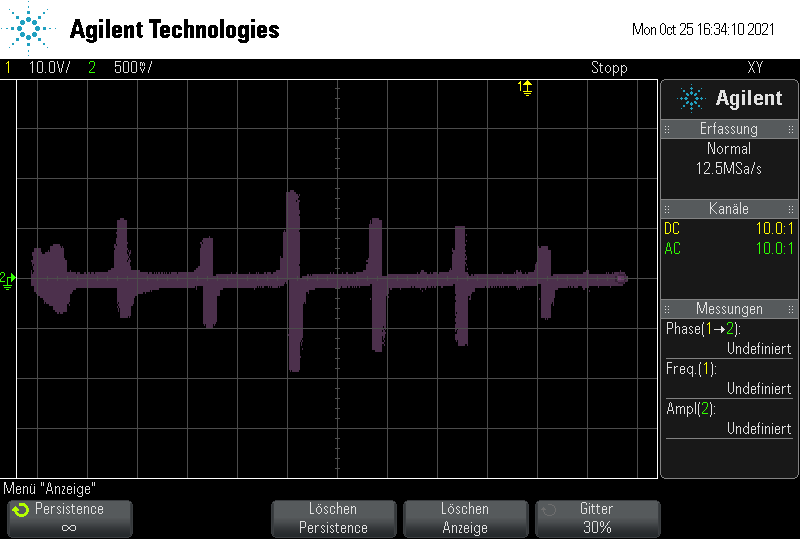
\includegraphics[width=\textwidth]{data/1_1zylinder50mm/scope_2.png}
        \caption{Oszilloskop, 2 Zylinder ($50 \, \symup{mm}$).}
    \end{subfigure}
    \hfill
    \begin{subfigure}[b]{0.3\textwidth}
        \centering
        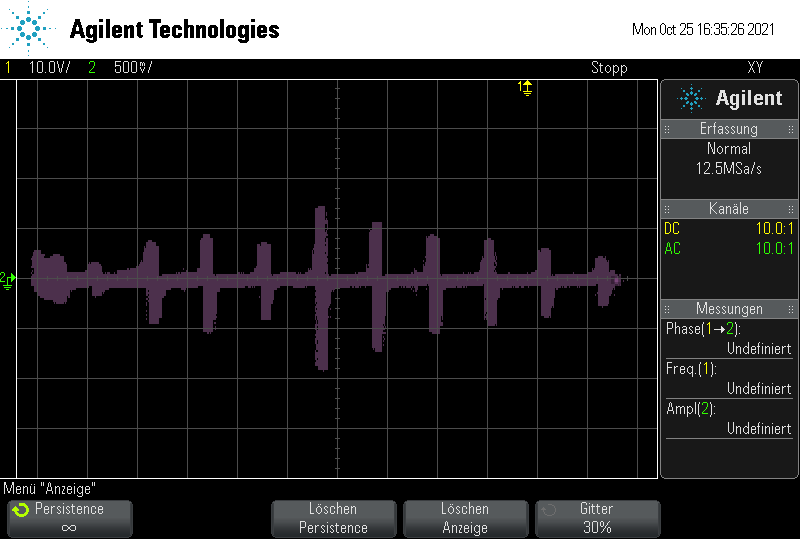
\includegraphics[width=\textwidth]{data/1_1zylinder50mm/scope_3.png}
        \caption{Oszilloskop, 3 Zylinder ($50 \, \symup{mm}$).}
    \end{subfigure}
    \hfill
    \begin{subfigure}[b]{0.3\textwidth}
        \centering
        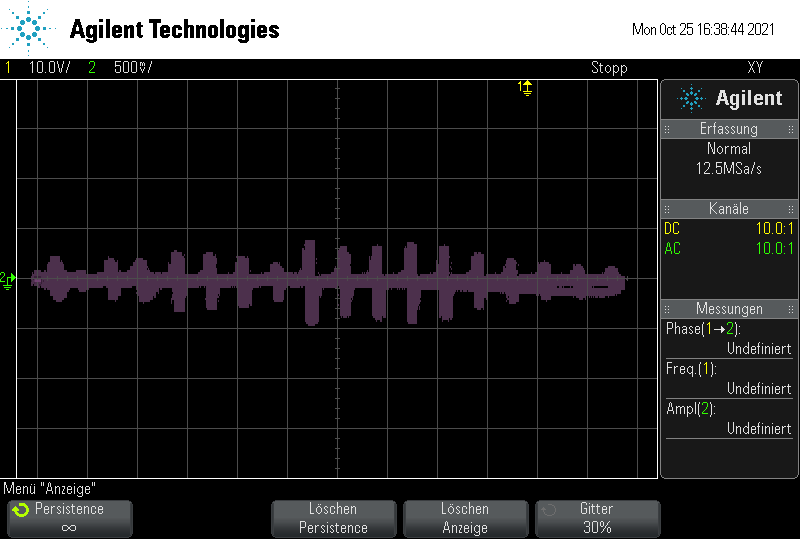
\includegraphics[width=\textwidth]{data/1_1zylinder50mm/scope_5.png}
        \caption{Oszilloskop, 5 Zylinder ($50 \, \symup{mm}$).}
    \end{subfigure}
    \hfill
    \begin{subfigure}[b]{0.3\textwidth}
        \centering
        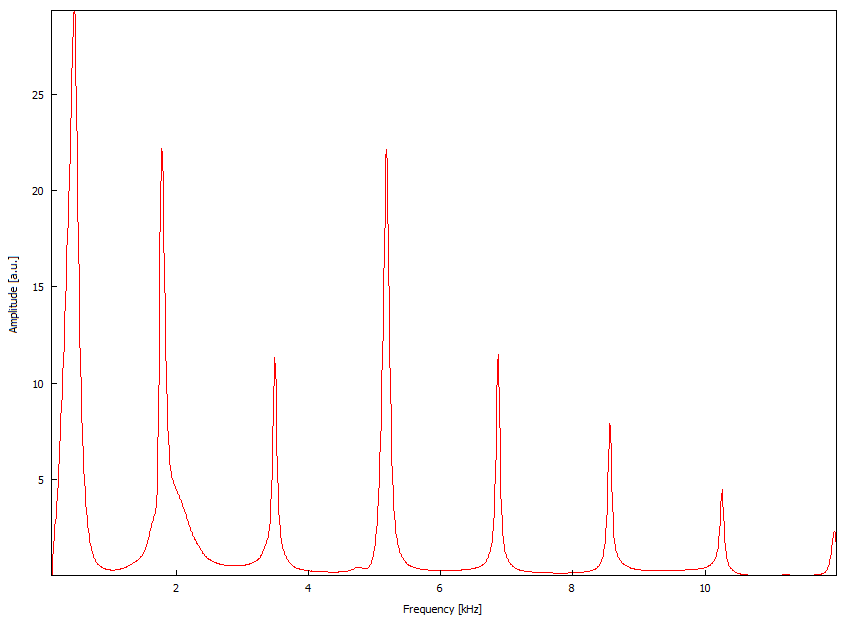
\includegraphics[width=\textwidth]{data/1_2zylinder50mmPC/2.png}
        \caption{PC, 2 Zylinder ($50 \, \symup{mm}$).}
    \end{subfigure}
    \hfill
    \begin{subfigure}[b]{0.3\textwidth}
        \centering
        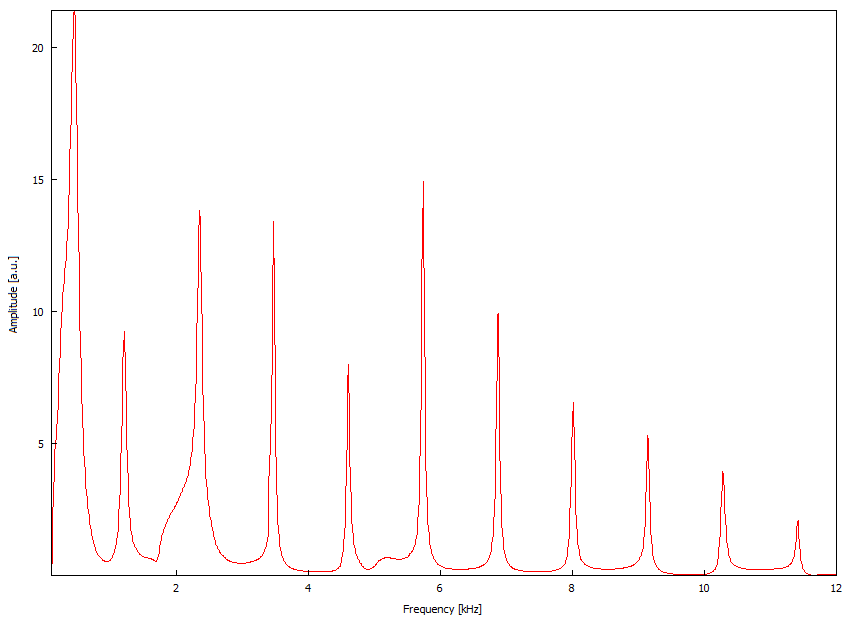
\includegraphics[width=\textwidth]{data/1_2zylinder50mmPC/3.png}
        \caption{PC, 3 Zylinder ($50 \, \symup{mm}$)}
    \end{subfigure}
    \hfill
    \begin{subfigure}[b]{0.3\textwidth}
        \centering
        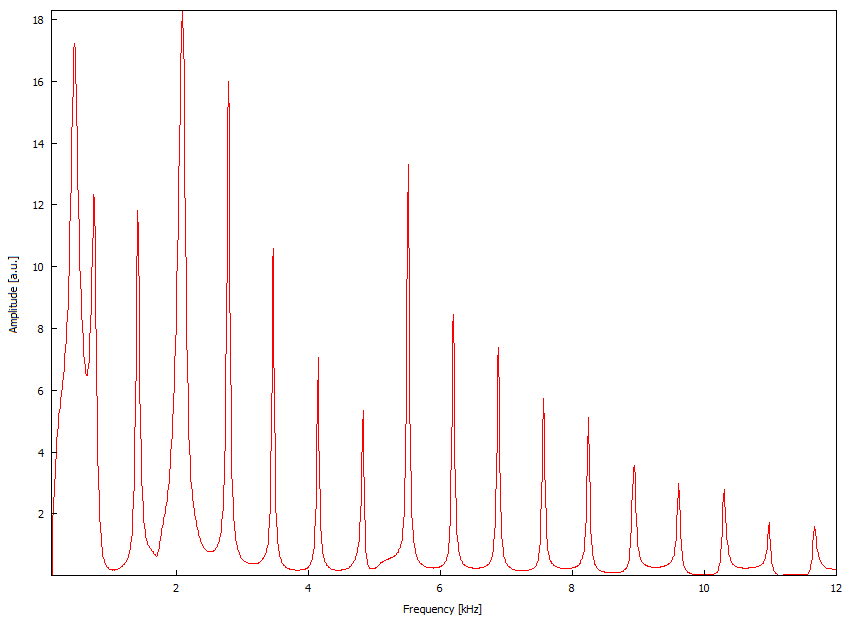
\includegraphics[width=\textwidth]{data/1_2zylinder50mmPC/5.png}
        \caption{PC, 5 Zylinder ($50 \, \symup{mm}$)}
    \end{subfigure}
       \caption{Das Frequenzspektrum von $0,1 \, \symup{kHz}$ bis $12 \, \symup{kHz}$ bei verschiedener Anzahlen Zylinder (Länge $50 \, \symup{mm}$) aufgenommen einmal mit einem Oszilloskop und einmal mit dem PC.}
       \label{fig:anhang1}
\end{figure}
\begin{figure}
    \centering
    \begin{subfigure}[b]{0.3\textwidth}
        \centering
        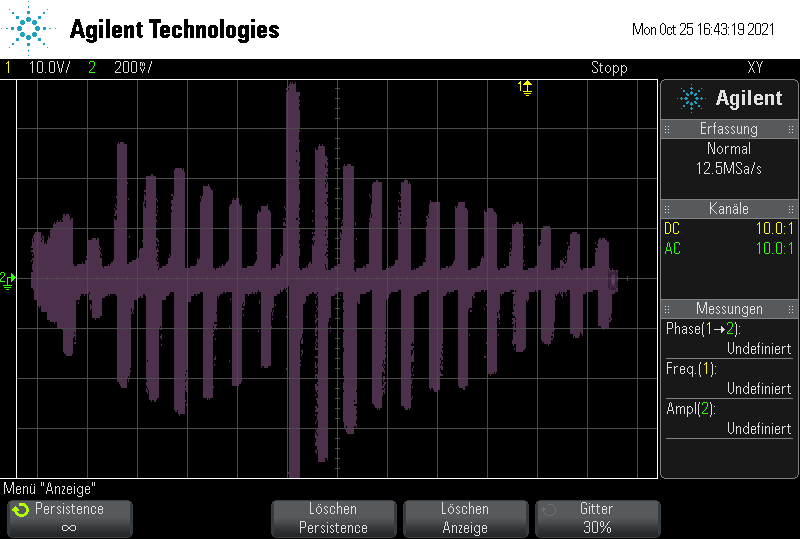
\includegraphics[width=\textwidth]{data/1_1zylinder50mm/scope_6.png}
        \caption{Oszilloskop, 6 Zylinder ($50 \, \symup{mm}$).}
    \end{subfigure}
    \hfill
    \begin{subfigure}[b]{0.3\textwidth}
        \centering
        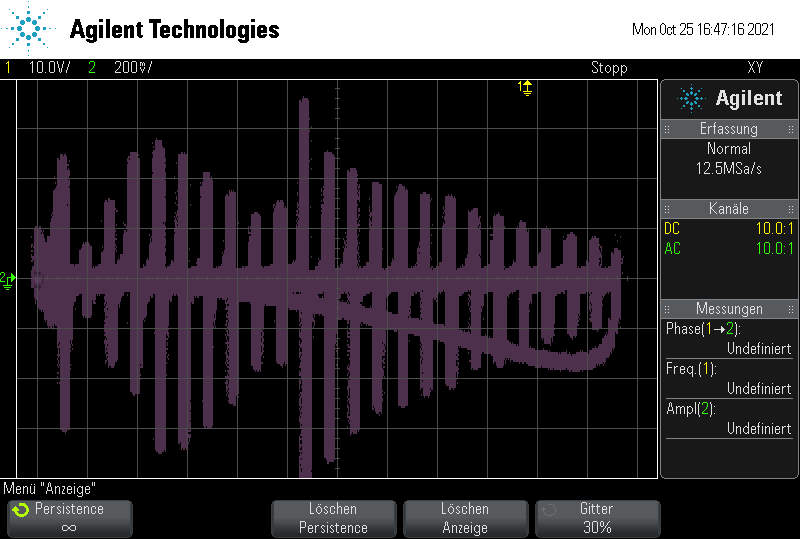
\includegraphics[width=\textwidth]{data/1_1zylinder50mm/scope_7.png}
        \caption{Oszilloskop, 7 Zylinder ($50 \, \symup{mm}$).}
    \end{subfigure}
    \hfill
    \begin{subfigure}[b]{0.3\textwidth}
        \centering
        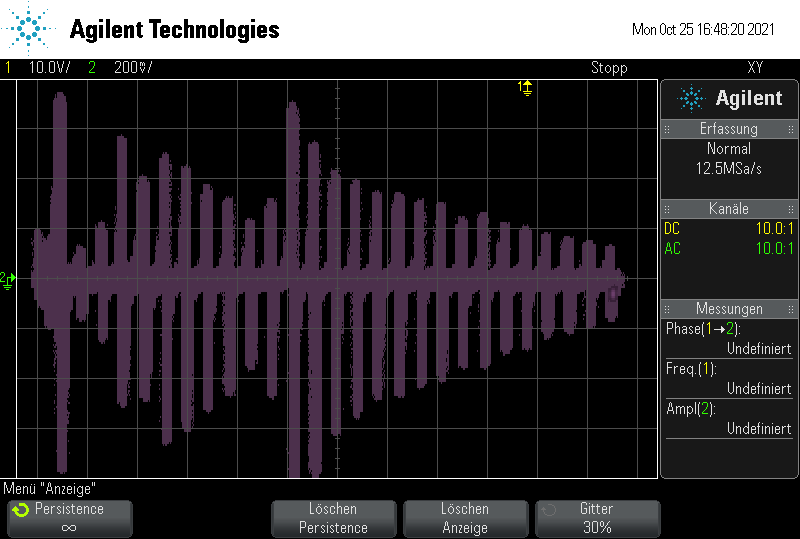
\includegraphics[width=\textwidth]{data/1_1zylinder50mm/scope_8.png}
        \caption{Oszilloskop, 8 Zylinder ($50 \, \symup{mm}$).}
    \end{subfigure}
    \hfill
    \begin{subfigure}[b]{0.3\textwidth}
        \centering
        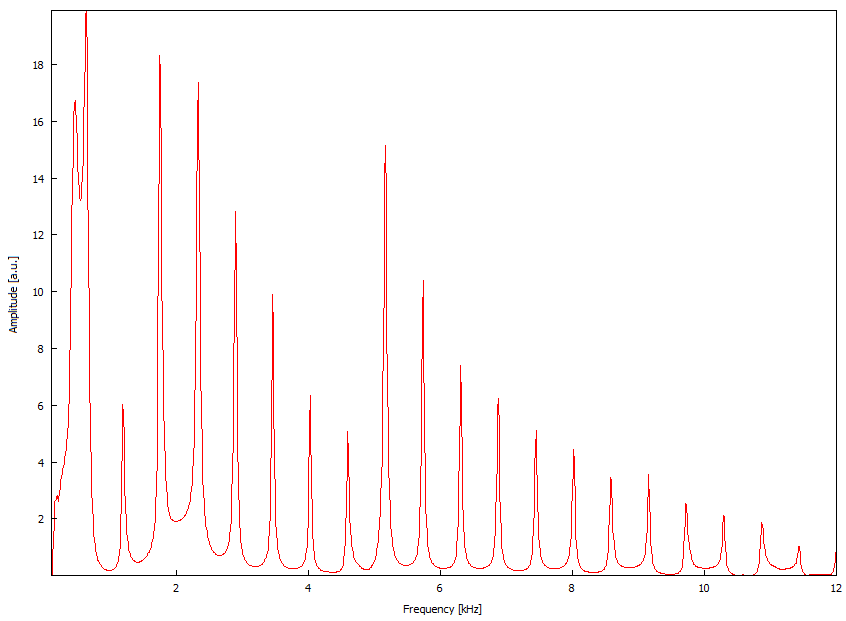
\includegraphics[width=\textwidth]{data/1_2zylinder50mmPC/6.png}
        \caption{PC, 6 Zylinder ($50 \, \symup{mm}$).}
    \end{subfigure}
    \hfill
    \begin{subfigure}[b]{0.3\textwidth}
        \centering
        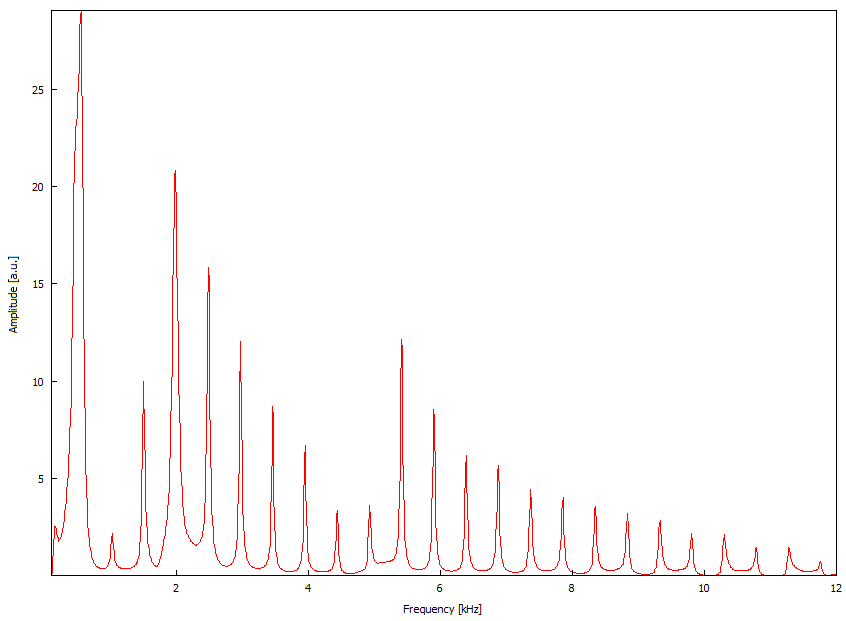
\includegraphics[width=\textwidth]{data/1_2zylinder50mmPC/7.png}
        \caption{PC, 7 Zylinder ($50 \, \symup{mm}$)}
    \end{subfigure}
    \hfill
    \begin{subfigure}[b]{0.3\textwidth}
        \centering
        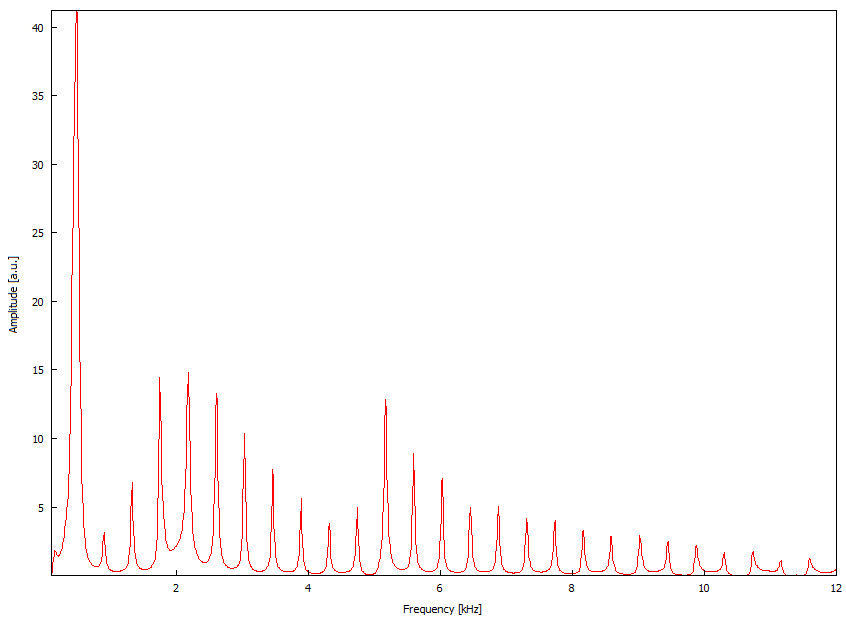
\includegraphics[width=\textwidth]{data/1_2zylinder50mmPC/8.png}
        \caption{PC, 8 Zylinder ($50 \, \symup{mm}$)}
    \end{subfigure}
       \caption{Das Frequenzspektrum von $0,1 \, \symup{kHz}$ bis $12 \, \symup{kHz}$ bei verschiedener Anzahlen Zylinder (Länge $50 \, \symup{mm}$) aufgenommen einmal mit einem Oszilloskop und einmal mit dem PC.}
       \label{fig:anhang2}
\end{figure}

\begin{figure}
    \centering
    \begin{subfigure}[b]{0.3\textwidth}
        \centering
        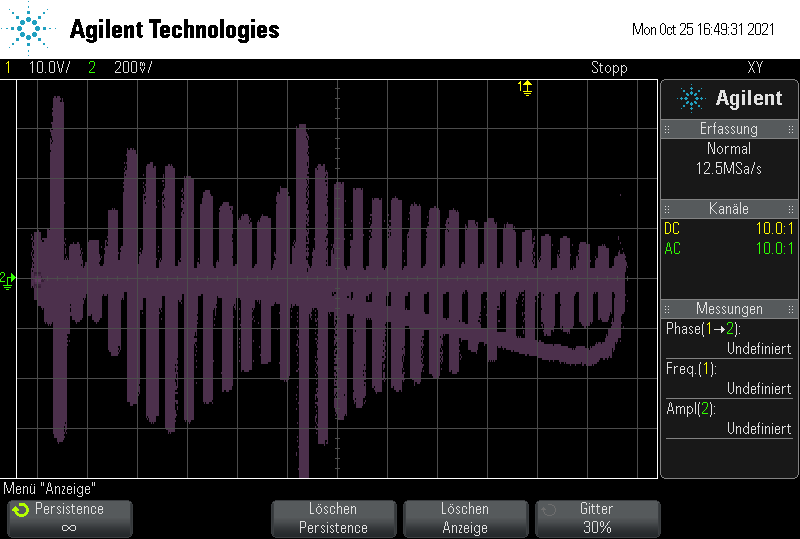
\includegraphics[width=\textwidth]{data/1_1zylinder50mm/scope_9.png}
        \caption{Oszilloskop, 9 Zylinder ($50 \, \symup{mm}$).}
    \end{subfigure}
    \hfill
    \begin{subfigure}[b]{0.3\textwidth}
        \centering
        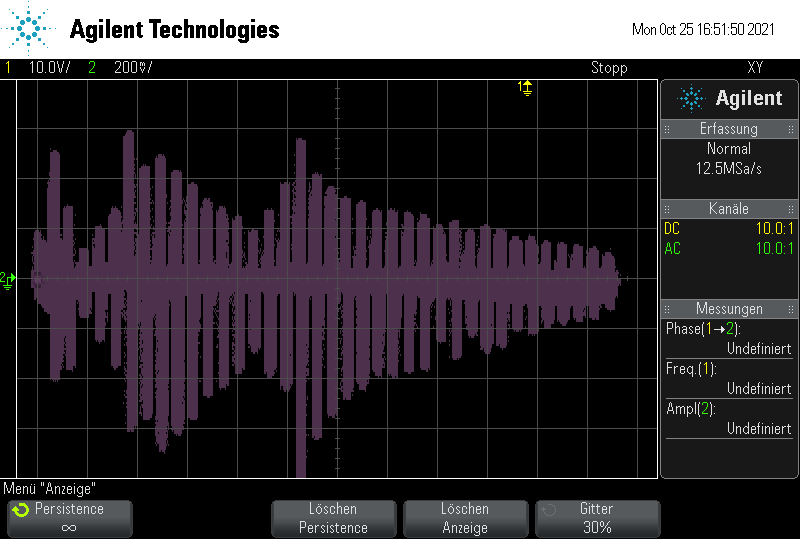
\includegraphics[width=\textwidth]{data/1_1zylinder50mm/scope_11.png}
        \caption{Oszilloskop, 11 Zylinder ($50 \, \symup{mm}$).}
    \end{subfigure}
    \hfill
    \begin{subfigure}[b]{0.3\textwidth}
        \centering
        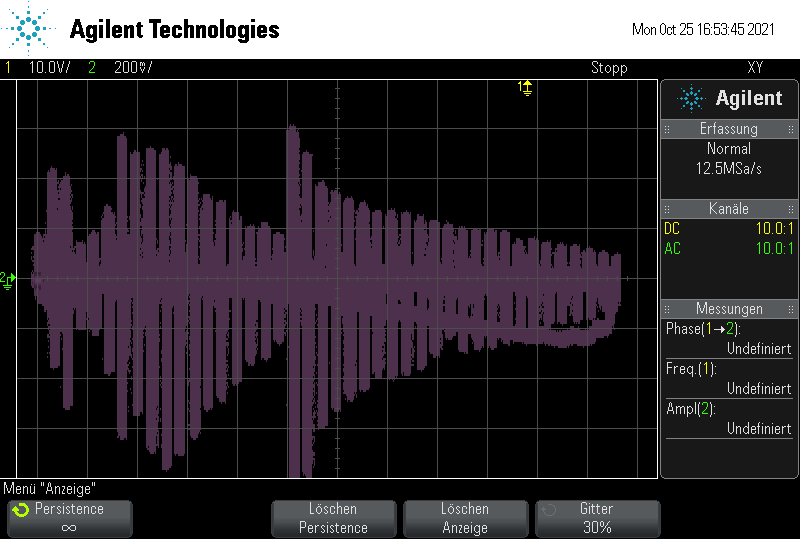
\includegraphics[width=\textwidth]{data/1_1zylinder50mm/scope_12.png}
        \caption{Oszilloskop, 12 Zylinder ($50 \, \symup{mm}$).}
    \end{subfigure}
    \hfill
    \begin{subfigure}[b]{0.3\textwidth}
        \centering
        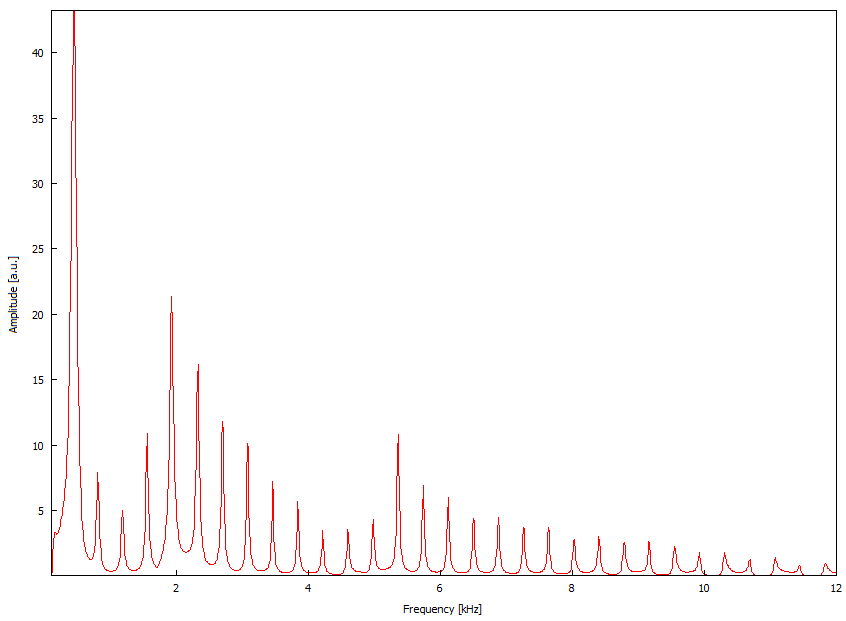
\includegraphics[width=\textwidth]{data/1_2zylinder50mmPC/9.png}
        \caption{PC, 9 Zylinder ($50 \, \symup{mm}$).}
    \end{subfigure}
    \hfill
    \begin{subfigure}[b]{0.3\textwidth}
        \centering
        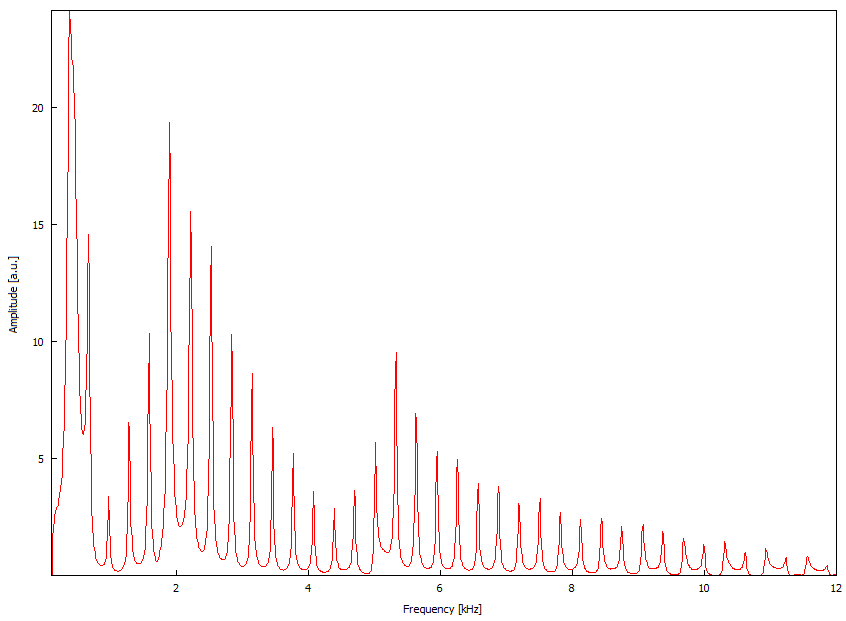
\includegraphics[width=\textwidth]{data/1_2zylinder50mmPC/11.png}
        \caption{PC, 11 Zylinder ($50 \, \symup{mm}$)}
    \end{subfigure}
    \hfill
    \begin{subfigure}[b]{0.3\textwidth}
        \centering
        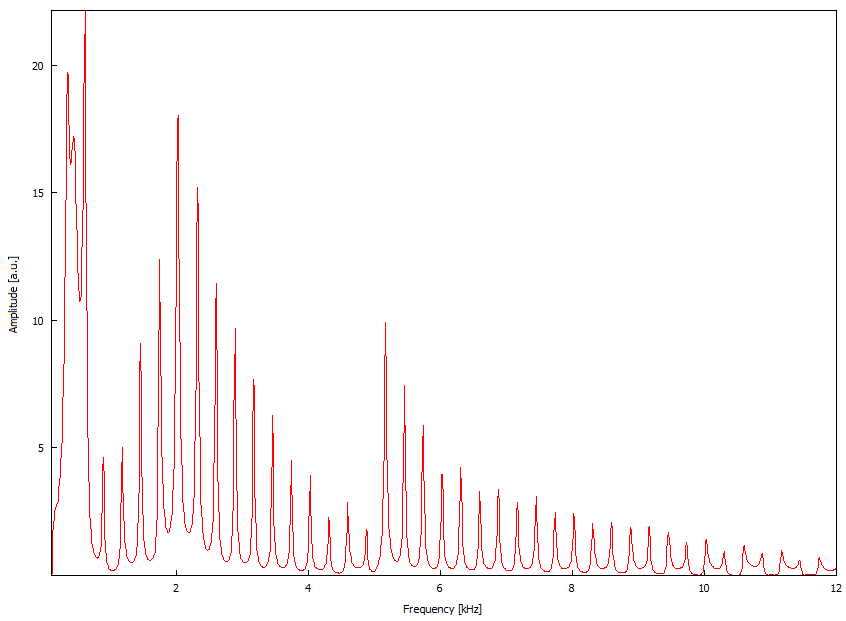
\includegraphics[width=\textwidth]{data/1_2zylinder50mmPC/12.png}
        \caption{PC, 12 Zylinder ($50 \, \symup{mm}$)}
    \end{subfigure}
       \caption{Das Frequenzspektrum von $0,1 \, \symup{kHz}$ bis $12 \, \symup{kHz}$ bei verschiedener Anzahlen Zylinder (Länge $50 \, \symup{mm}$) aufgenommen einmal mit einem Oszilloskop und einmal mit dem PC.}
       \label{fig:anhang3}
\end{figure}

\begin{figure}
    \centering
    \begin{subfigure}[b]{0.3\textwidth}
        \centering
        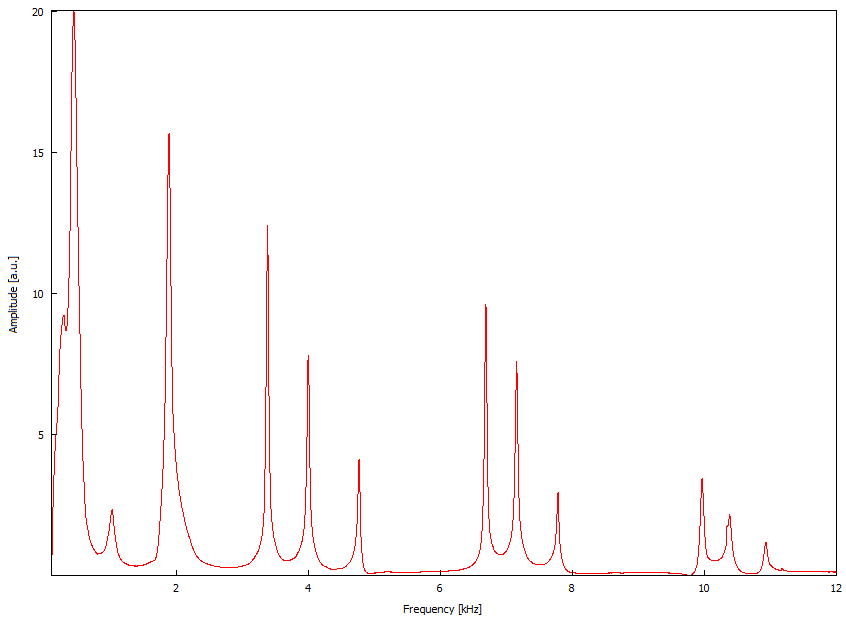
\includegraphics[width=\textwidth]{data/4_1/3.png}
        \caption{3 Zylinder.}
    \end{subfigure}
    \hfill
    \begin{subfigure}[b]{0.3\textwidth}
        \centering
        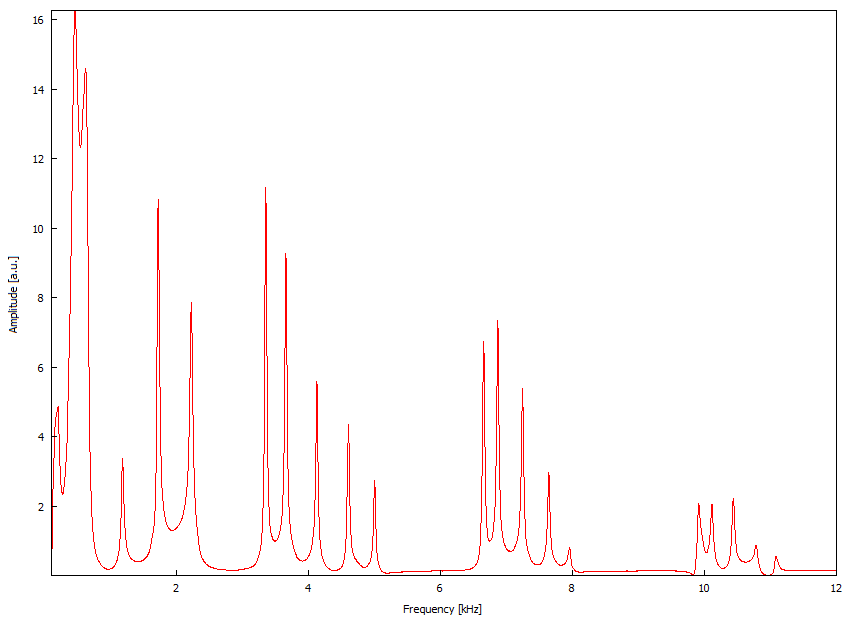
\includegraphics[width=\textwidth]{data/4_1/5.png}
        \caption{5 Zylinder.}
    \end{subfigure}
    \hfill
    \begin{subfigure}[b]{0.3\textwidth}
        \centering
        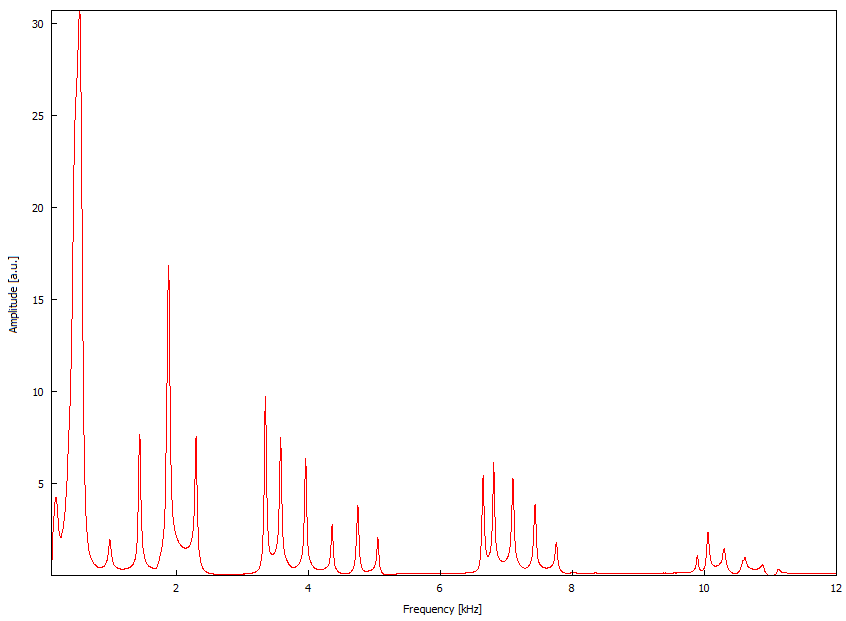
\includegraphics[width=\textwidth]{data/4_1/6.png}
        \caption{6 Zylinder.}
    \end{subfigure}
    \hfill
    \begin{subfigure}[b]{0.3\textwidth}
        \centering
        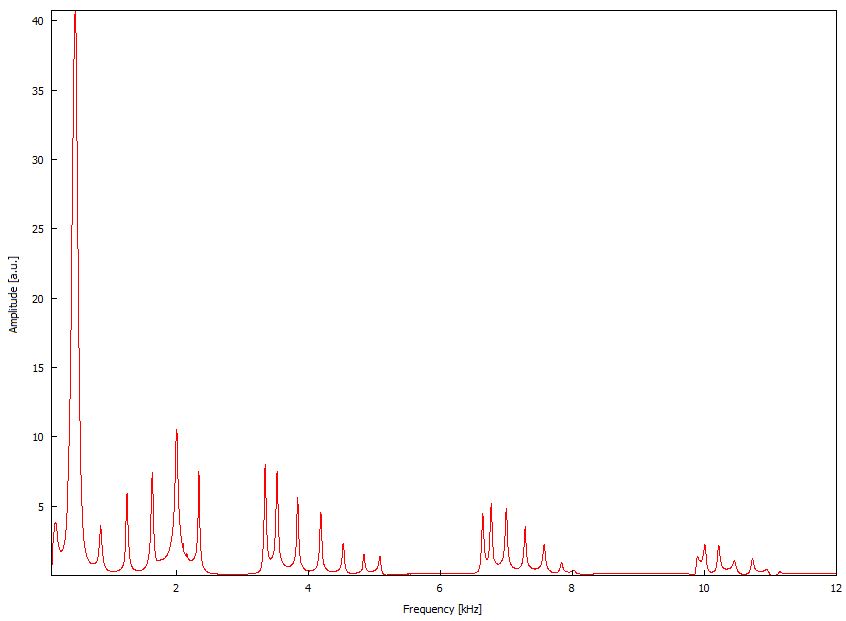
\includegraphics[width=\textwidth]{data/4_1/7.png}
        \caption{3 Zylinder.}
    \end{subfigure}
    \hfill
    \begin{subfigure}[b]{0.3\textwidth}
        \centering
        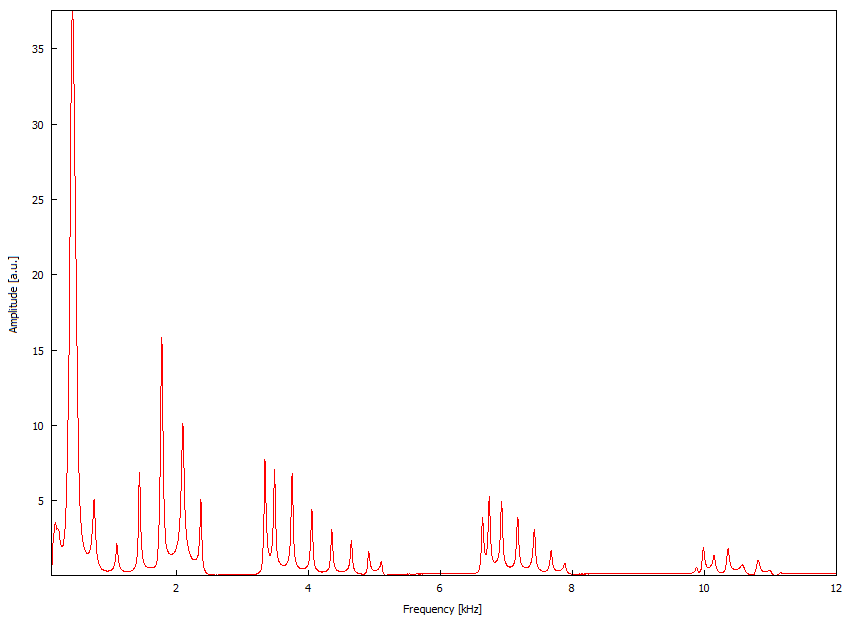
\includegraphics[width=\textwidth]{data/4_1/8.png}
        \caption{5 Zylinder.}
    \end{subfigure}
    \hfill
    \begin{subfigure}[b]{0.3\textwidth}
        \centering
        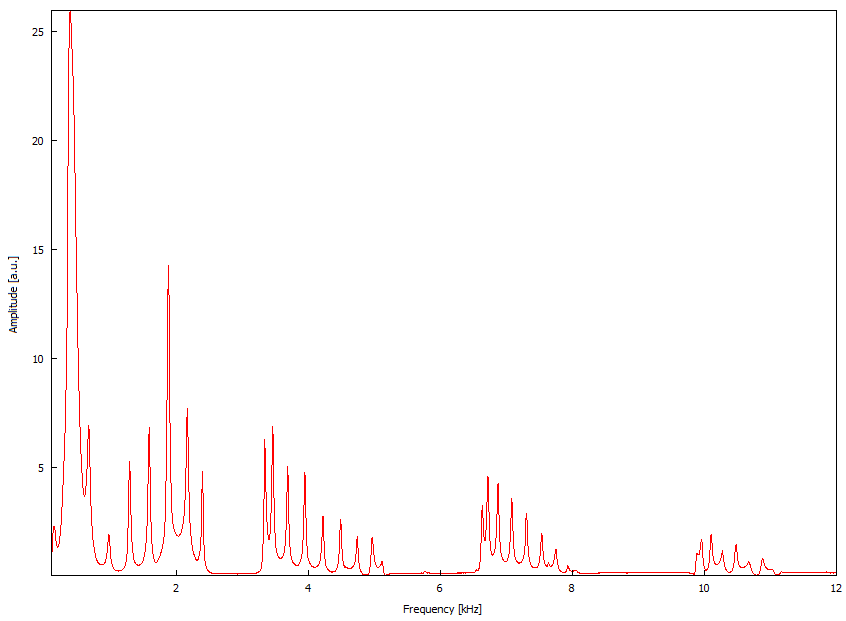
\includegraphics[width=\textwidth]{data/4_1/9.png}
        \caption{6 Zylinder.}
    \end{subfigure}
    \hfill
    \caption{Frequenzspektrum von verschiedenen Anzahlen Zylinder mit 50\;mm Länge und jeweils Irsiblenden mit 16\;mm Durchmesser dazwischen im Bereich 0,1\;kHz bis 12\;Hz.}
    \label{fig:anhang_allesgleich}
\end{figure}